\documentclass[11pt]{article}

%Afegim els "packages" necessaris per generar el document
\usepackage[utf8]{inputenc}
\usepackage{graphicx}
\usepackage{fancyhdr}
\usepackage{hyperref}
\usepackage{tocloft}
\usepackage[T1]{fontenc}


\title{Instal·lació Code-Lite (Linux)}
\author{Autor: Albert Lloveras Carbonell\\Revisió: Joaquim Porte Rodríguez}
\date{}

\renewcommand\contentsname{\huge Índex \vspace{8pt} \hrule}
\renewcommand{\cftsecleader}{\cftdotfill{\cftdotsep}}

%------------------------------------------------------------
%	Definició de Capçaleres i Peus de Pàgina
%------------------------------------------------------------

\fancypagestyle{pageStyle}{
	%Definim la capçalera de l'esquerra (Logo Salle)
	\fancyhead[L]{
		
\includegraphics[scale=0.25]{img/la_salle_logo.jpg}
	} 

	%Definim la capçalera de la dreta (Info Curs i Assignatura)
	\fancyhead[R]{
		\vtop{
			Manual d'instal·lació\\
			Code-Lite (Ubuntu)\\
		}
	}
	\fancyfoot[C]{} %Peu de pàgina central
	\fancyfoot[L]{Departament d'Enginyeria - Informàtica} %Peu de pàgina esquerra
	\fancyfoot[R]{\thepage} %Peu de pàgina dreta (Número de pàgina)	
	%Configuracions extra
	\renewcommand{\headrulewidth}{0pt} %Ocultem la línia de separació entre 		capçalera i bloc de text
	\renewcommand{\footrulewidth}{2pt} %Fixem la línia de separació entre peu de pàgina i bloc de text
	\setlength{\headheight}{67pt} %Fixem la mida de la capçalera	
	
}

%Definim la macro (nofooter) per poder amagar el peu de pàgina quan interessi
\fancypagestyle{nofooter}{
	\fancyfoot{}
	\renewcommand{\footrulewidth}{0pt}
}

%Definim la macro (nofooter) per poder amagar el peu de pàgina quan interessi
\fancypagestyle{empty}{
	\fancyfoot{}
	\fancyhead{}
	\renewcommand{\footrulewidth}{0pt}
	\renewcommand{\headrulewidth}{0pt}
}

\begin{document}

\pagestyle{empty}
\begin{center}

	%--- Logo de la portada --- %
	
\includegraphics[width=0.15\textwidth]{img/code-lite.png}~\\[1cm]
	
	%---- Nom del programa --- %
	\textsc{\LARGE Code-Lite}\\[1.5cm]
	
	%-- Nom del manual -- %
	\hrule
	\vspace{8pt}
	\huge{\bfseries Manual d'instal·lació (Ubuntu)}
	\vspace{8pt}
	\hrule	
	\vspace{12pt	}

	% -- Nom de l'autor i del supervisor
	\noindent
	\begin{minipage}{0.4\textwidth}
		\begin{flushleft} \large
			\emph{Autor:}\\
			Albert \textsc{Lloveras}
		\end{flushleft}
	\end{minipage}%
	\begin{minipage}{0.4\textwidth}
		\begin{flushright} \large
			\emph{Revisió:} \\
			Joaquim \textsc{Porte}
		\end{flushright}
	\end{minipage}
	\vfill

\end{center}

%---- Índex ---- %
\newpage

\pagestyle{empty}
\tableofcontents


%---- Començament del document --- %
\newpage
\pagestyle{pageStyle}


\section{Introducció}
En aquest manual es donaran les pautes per a la instal·lació de Code-Lite al vostre ordinador. Code-Lite és un entorn de desenvolupament integrat que permet el desenvolupament de projectes de programació d'una manera més àgil i pràctica que des del terminal, ja que és un processador de textos especialitzat en codi C. D'aquesta manera, se'ns prestaran certes ajudes mentre codifiquem que ens permetran accelerar el procés de desenvolupament. \linebreak \linebreak
\textbf{Nota important:} Aquesta guia està enfocada a tothom que utilitzi Ubuntu 14 al seu ordinador ja que amb altres sistemes operatius o versions inferiors d'Ubuntu alguns passos de la instal·lació podrien no funcionar.


\section{Preparació de l'ordinador i obtenció del software}
\noindent En primer lloc haurem de realitzar una sèrie de canvis al nostre ordinador per tal de que Code-Lite es pugui instal·lar correctament al nostre ordinador. Per començar, haurem d'obrir una finestra del Terminal d'Ubuntu. Per fer-ho, podem prémer la combinació de tecles \textbf{Control + Alt + T} i ens apareixerà la següent finestra:

\begin{center}
	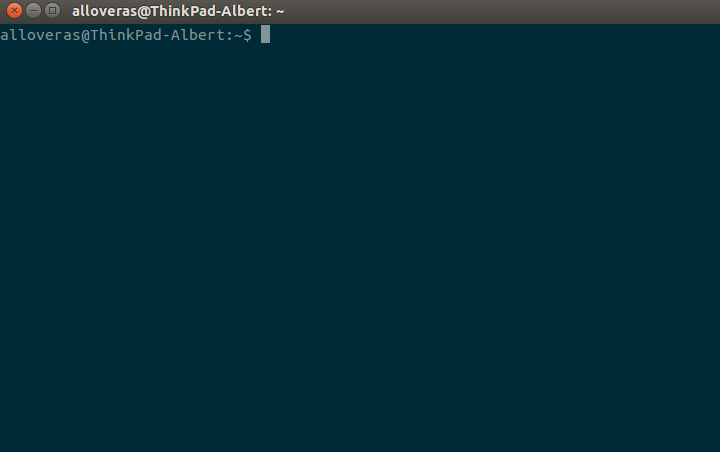
\includegraphics[scale=0.4]{img/Ubuntu_Terminal_Screen.png}
\end{center}

\noindent En aquesta finestra serà on escriurem les següents comandes per tal de deixar apunt el nostre ordinador preparat per la instal·lació de Code-Lite.\pagebreak

\noindent En primer lloc, haurem d'instal·lar el paquet \textbf{build-essentials} d'Ubuntu per tal de garantir que tenim els compiladors i les llibreries estàndards per a l'elaboració de projectes basats en els llenguatges C/C++. Per fer-ho, executarem la següent comanda al terminal que acabem d'obrir:

\begin{center}
	\textbf{sudo apt-get install build-essential}
\end{center}

\begin{center}
	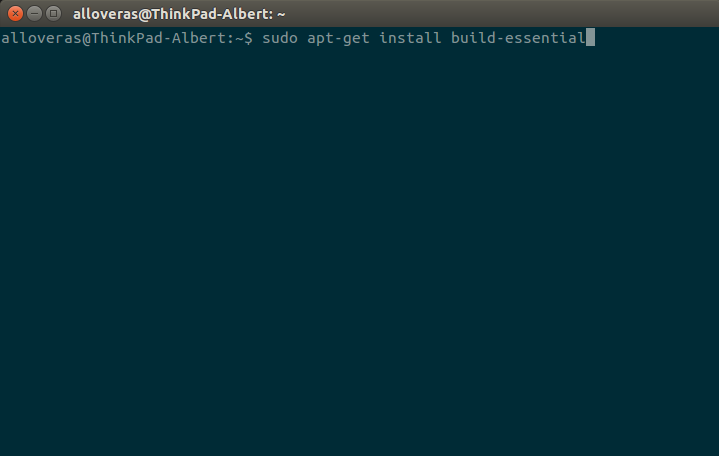
\includegraphics[scale=0.4]{img/Build_Essential_Install.png}
\end{center}

\noindent \textbf{Nota:} Se'ns demanarà la clau d'administrador per executar la comanda ja que aquesta conté la directiva \textbf{sudo} la qual només pot ser usada per administradors se l'ordinador. La clau no es mostrarà mentre s'està escrivint per raons de seguretat. Un cop acabada d'escriure només caldrà prémer ENTER per confirmar la introducció encara que no hagi aparegut res a la pantalla. Si la introducció és correcte, el procés continuarà, sinó, se'ns tornarà a demanar la clau. \\

\noindent En segon lloc, haurem de localitzar el nom de la nostre distribució d'Ubuntu. Per fer-ho escriurem al terminal:
\begin{center}
	\textbf{lsb\_release -a}
\end{center}

\pagebreak
\noindent Si tot va bé ens hauria de sortir un missatge com el següent de qual només ens hem de fixar en la línia que ens diu quin es el \textbf{CodeName} de la nostre versió d'Ubuntu.
\begin{center}
	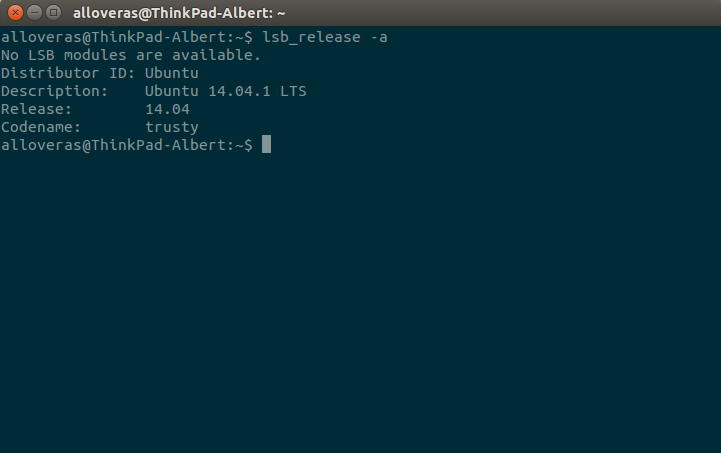
\includegraphics[scale=0.3]{img/Ubuntu_Code_Name.png}
\end{center}
\noindent En el nostre cas, el nom de la nostre versió d'Ubuntu és \textbf{trusty} però això pot variar en cada ordinador. De totes maneres, si s'està usant una versió d'Ubuntu superior a la 14.04, totes les que apareguin seran vàlides per a la instal·lació de Code-Lite a través d'aquesta guia. \\

\noindent Un cop obtingut el nom de la nostre versió, ens podem disposar a la descàrrega i instal·lació de Code-Lite. Per fer-ho executarem les següents comandes:
\begin{center}
	\small{\textbf{sudo apt-key adv --fetch-keys http://repos.codelite.org/CodeLite.asc}}
\end{center}

\begin{center}
	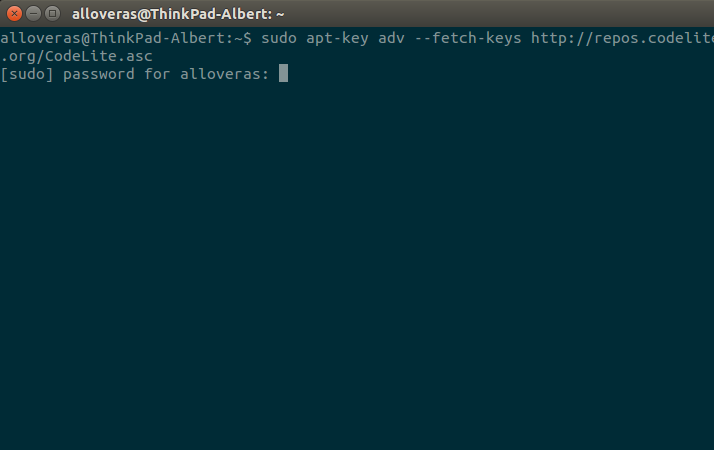
\includegraphics[scale=0.3]{img/Add_Repository_Keys.png}
\end{center}

\pagebreak
\noindent Un cop fet això, haurem de triar de la següent llista la comanda a executar ja que aquesta serà diferent en funció del nom de la versió d'Ubuntu que haguem obtingut anteriorment:

\begin{center}
	\begin{tabular}{||l|l||}
		\hline
		\hline
		Nom Versió & Comanda \\
		\hline
		Wheezy & sudo apt-add-repository 'deb 				http://repos.codelite.org/debian/ wheezy contrib' \\
		\hline
		Saucy & sudo apt-add-repository 'deb http://repos.codelite.org/ubuntu/ saucy universe'\\
		\hline
Trusty & sudo apt-add-repository 'deb http://repos.codelite.org/ubuntu/ trusty universe'\\
		\hline
		\hline
	\end{tabular}
\end{center}

\noindent Al executar una de les comandes anteriors se'ns tornarà a demanar la introducció de la clau d'administrador perquè la comanda torna a incloure la directiva \textbf{sudo} de manera que l'haurem de tornar a introduir per que s'executi completament.\\ A continuació es mostra un exemple de l'execució de la comanda:
\begin{center}
	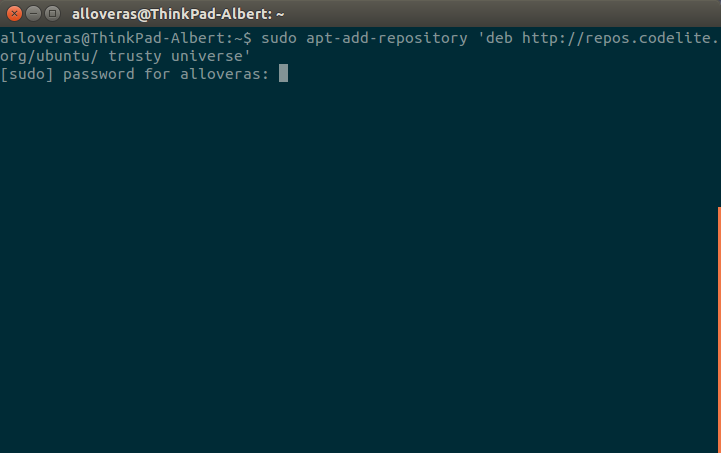
\includegraphics[scale=0.4]{img/Add_Repository.png}
\end{center}

\pagebreak
\noindent Un cop fet això, ens caldrà obligar a Ubuntu a registrar els nous repositoris que acabem d'afegir. Per fer-ho, n'hi haurà prou en executar la següent comanda:
\begin{center}
	\textbf{sudo apt-get update}
\end{center}

\begin{center}
	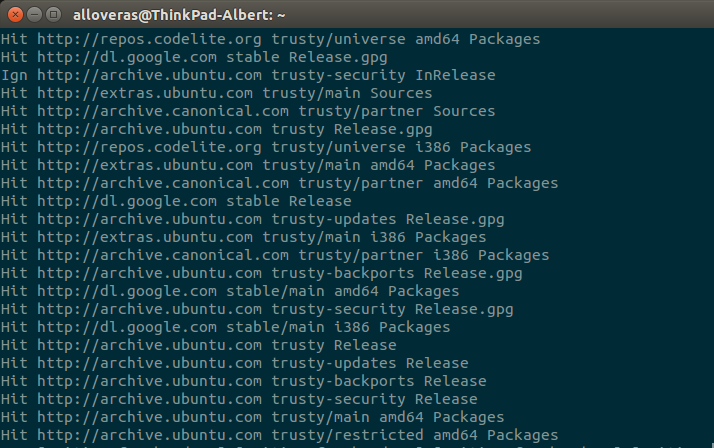
\includegraphics[scale=0.4]{img/Apt_Get_Update.png}
\end{center}

\noindent \textbf{Nota:} En aquesta comanda se'ns tornarà a demanar la introducció de la clau d'administrador.\\

\noindent Un cop completada la comanda anterior, ja ens podem disposar a realitzar la instal·lació per mitjà de l'execució de la següent comanda:
\begin{center}
	\textbf{sudo apt-get install codelite wxcrafter}
\end{center}

\noindent Abans de començar la instal·lació, se'ns demanarà la confirmació abans de continuar tal i com es mostra en la imatge següent. Cal contestar \textbf{Sí} a la pregunta escrivint \textbf{s} o \textbf{y} en funció de si tenim Ubuntu en (Català / Castellà) o en anglès. Un cop acabada la instal·lació, ja podrem usar Code-Lite per primera vegada. 

\begin{center}
	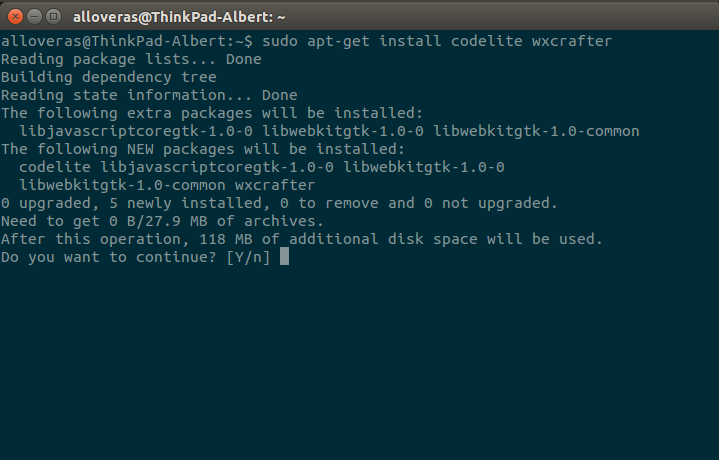
\includegraphics[scale=0.4]{img/Apt_Get_Install.png}
\end{center}

\noindent \textbf{Nota:} En aquesta comanda se'ns tornarà a demanar la introducció de la clau d'administrador.

\section{Obertura i Configuracions de Code-Lite}
Ara que ja disposem de Code-Lite al nostre ordinador ens disposarem a realitzar les configuracions inicials per tal de que puguem començar a treballar en els nostres projectes. Per començar, obrirem el el programa per primer cop mitjançant l'ús de la comanda següent al terminal:
\begin{center}
	\textbf{codelite}
\end{center}
\begin{center}
	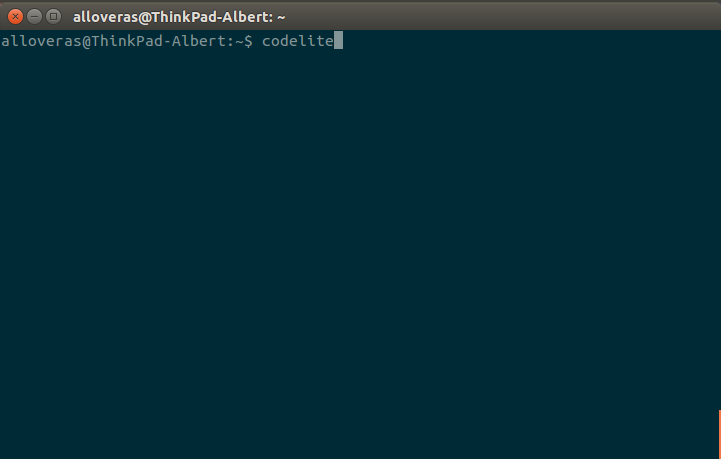
\includegraphics[scale=0.4]{img/CodeLite_First_Opening.png}
\end{center}

\pagebreak \noindent Si tot va com s'espera, una finestra com la següent ens hauria d'aparèixer:

\begin{center}
	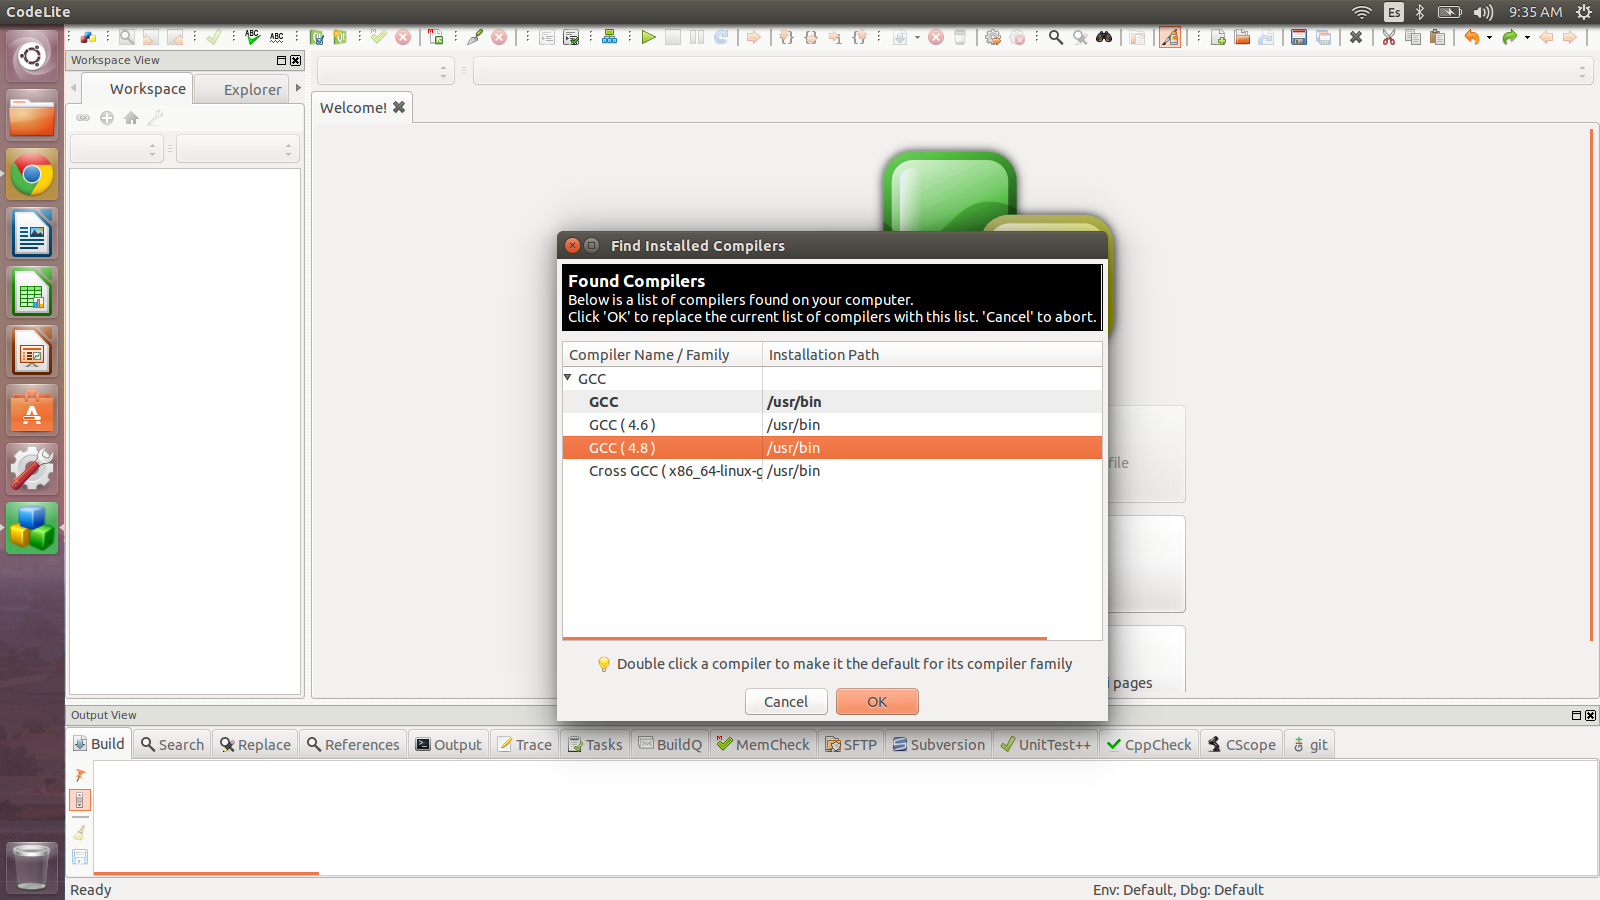
\includegraphics[scale=0.25]{img/Compiler_Selection_CodeLite.png}
\end{center}

\noindent En aquesta finestra haurem de seleccionar el compilador que voldrem que CodeLite utilitzi alhora de compilar els nostres projectes. Haurem de seleccionar el \textbf{GCC} i en cas de que estigui disponible, la opció que diu \textbf{GCC (4.8)} tot i que tampoc és indispensable tenir la última versió del compilador però sí molt recomanable. \\

\noindent Un cop fet això, ens trobarem a la finestra inicial de Code-Lite i estarem preparats per començar a crear i desenvolupar els nostres projectes de programació en C/C++.


\end{document}